%!TEX root = ../main.tex

\begin{frame}{Resultados Parciais}
 \begin{itemize}
   \item Estimação de idade a partir de uma imagem de face
   \ \ \newline
    \item Arquiteturas
    \begin{itemize}
      \item LeNet
      \item AlexNet
      \item VGG-16
      \item SqueezeNet
    \end{itemize}
   \ \ \newline
   \item \alert{9 Abordagens}
   \end{itemize}
\end{frame}


\begin{frame}{Abordagem 1}
 \begin{itemize}
   \item Entradas: Imagens normalizadas
   \item Redes: LeNet e AlexNet
   \item Funções de ativação: \emph{ReLU} e \emph{Leaky ReLU}
   \end{itemize}
\end{frame}

\begin{frame}{Abordagem 1}
\begin{figure}[h!]
  \caption{Resultados do treinamento e teste da CNN LeNet de acordo com a Abordagem 1.}\label{fig:lenet-abordagem1}
  \begin{subfigure}[hb]{0.25\linewidth}
    \caption{RMSE de treinamento da arquitetura LeNet utilizando funções de ativação \emph{ReLU}.}

    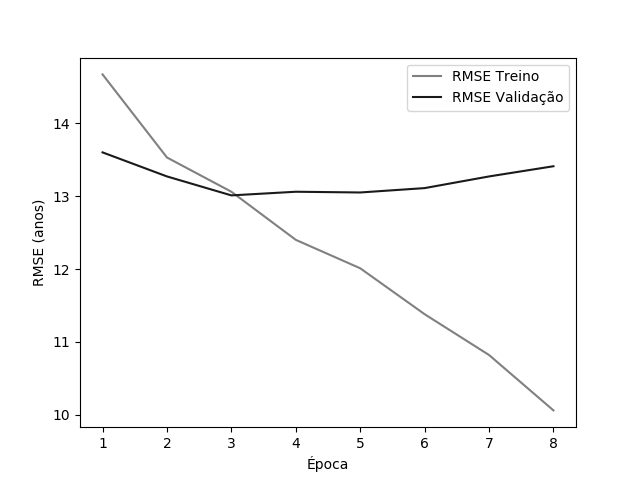
\includegraphics[width=\linewidth]{img/graficos/history/lenet/fig-history-image-treat-1-lenet-relu-rmse.png}%
  \end{subfigure}%
  \begin{subfigure}[hb]{0.25\linewidth}
    \caption{Reta-0 LeNet \emph{ReLU}.}

    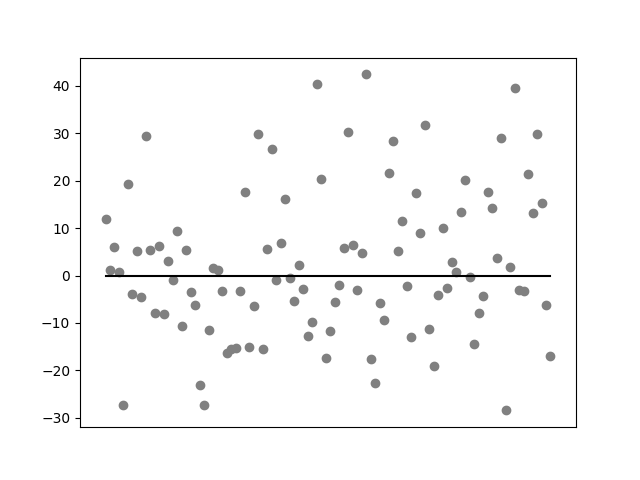
\includegraphics[width=\linewidth]{img/graficos/reta0/lenet/fig-reta-0-image-treat-1-lenet-relu.png}%
  \end{subfigure}
  \begin{subfigure}[hb]{0.25\linewidth}
    \caption{RMSE de treinamento da arquitetura LeNet utilizando funções de ativação \emph{Leaky ReLU}.}

    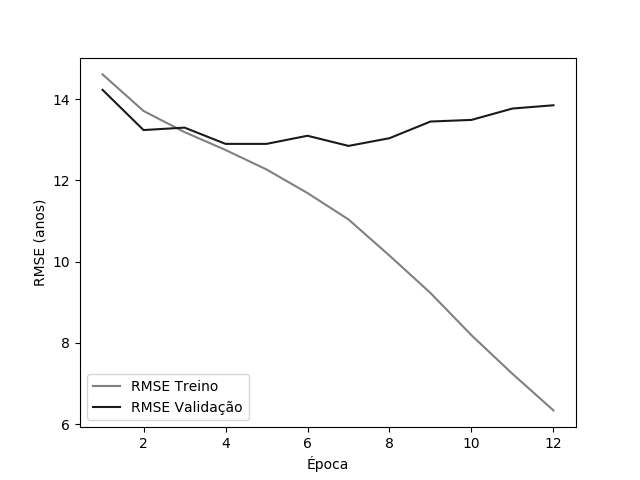
\includegraphics[width=\linewidth]{img/graficos/history/lenet/fig-history-image-treat-1-lenet-lrelu-rmse.png}
  \end{subfigure}
  \begin{subfigure}[hb]{0.25\linewidth}
    \caption{Reta-0 LeNet \emph{Leaky ReLU}.}

   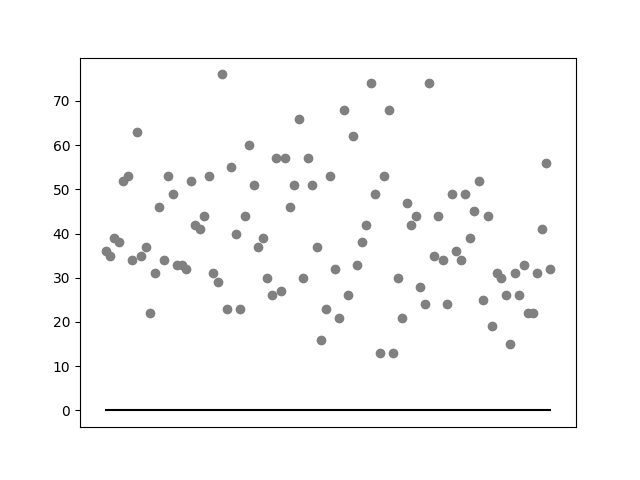
\includegraphics[width=0.25\linewidth]{img/graficos/reta0/lenet/fig-reta-0-image-treat-1-lenet-lrelu.png}
  \end{subfigure}%
\end{figure}
\end{frame}
